\documentclass[9pt]{article}
\usepackage[a5paper,hmargin=2.8cm,vmargin=2.5cm]{geometry}
\usepackage{xcolor}
\usepackage{ebgaramond}
\input GoudyIn.fd
\newcommand*\initfamily{\usefont{U}{GoudyIn}{xl}{n}}
\usepackage{wallpaper}

\pagestyle{empty}
\setlength\parindent{0pt}

\definecolor{dred}{HTML}{891d1d}
%\newcommand{\h}[1]{\textcolor{red!70!black}{#1}}
\newcommand{\h}[1]{\textcolor{dred}{#1}}
\newcommand{\g}[1]{\textcolor{black}{#1}}

% ---
\begin{document}

% add wallpaper
\CenterWallPaper{1}{tazhib-persa-c-48_2b}
\mbox{}

% top banner
\begin{center}
	\includegraphics[width=0.3\textwidth]{calli_dred}
\end{center}

\vspace{-2em}

\noindent\makebox[\linewidth][c]{
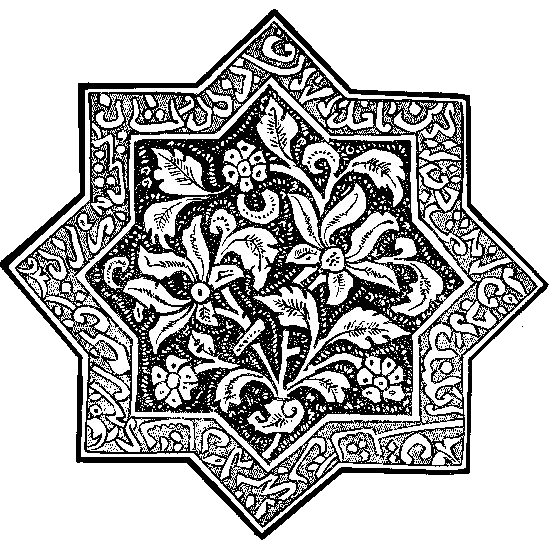
\includegraphics[width=0.2\textwidth]{star}
\hspace{7em}
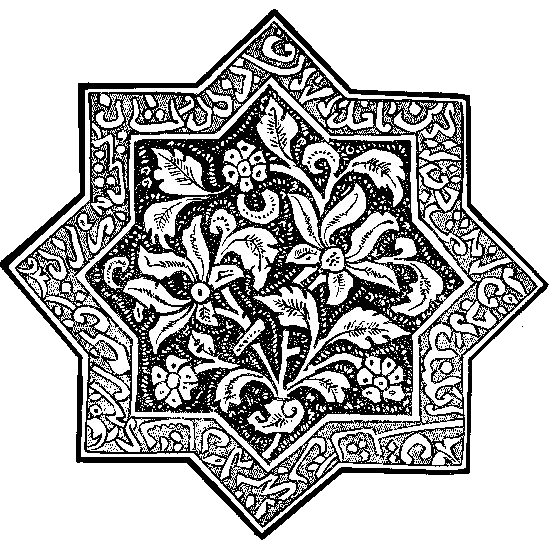
\includegraphics[width=0.2\textwidth]{star}
}

% title
\begin{center}
{\Huge {\textsc{\h{S}\g{elamat} \h{H}\g{ari} \h{R}\g{aya} \h{I}\g{dul} \h{F}\g{itri}\\[4pt]
\g{1446} \h{H}}}}\\
\end{center}

% body
\smallskip

\begin{center}
\g{Bersama ini kami,}
\end{center}
\begin{center}
\textsc{{\huge \h{M}}{\Large \g{o}} {\huge \h{W}}{\Large \g{i}}}\\
{\huge {\textsc{\h{\&}}}}\\[2pt]
\textsc{{\huge \h{H}}{\Large \g{o}} {\huge \h{S}}{\Large \g{e}}}\\
\end{center}
\smallskip

\g{mengucapkan selamat Hari Lebaran.
Semoga keberkahan dan kebahagiaan menyertai kita semua.}

\g{Mohon maaf lahir dan batin.}

% signature
\normalfont\initfamily
\begin{center}
\fontsize{12mm}{12mm}\selectfont \h{MW} \hfill \h{HS}
\end{center}

\end{document}

%Image sources:
%- frame https://fotografia.islamoriente.com/de/gallery/tazhib-cadre
%- calligraphy https://www.pngegg.com/en/png-bmtuk
%- star symbol https://syedfawaz2002.wordpress.com/2011/09/29/islamic-patterns-and-geometric-tessellations/persian-designs-33/
